%
% The first command in your LaTeX source must be the \documentclass command.
\documentclass[sigconf]{acmart}

%
% defining the \BibTeX command - from Oren Patashnik's original BibTeX documentation.
\def\BibTeX{{\rm B\kern-.05em{\sc i\kern-.025em b}\kern-.08emT\kern-.1667em\lower.7ex\hbox{E}\kern-.125emX}}  

 % Rights management information. 
% This information is sent to you when you complete the rights form.
% These commands have SAMPLE values in them; it is your responsibility as an author to replace
% the commands and values with those provided to you when you complete the rights form.
%
% These commands are for a PROCEEDINGS abstract or paper.
\copyrightyear{2019}
\acmYear{2019}
\setcopyright{acmlicensed}
\acmConference{N.A}
\acmBooktitle{N.A.}
\acmPrice{0.00}
\acmDOI{N.A}
\acmISBN{N.A.}

% end of the preamble, start of the body of the document source.
\begin{document}

%
% The "title" command has an optional parameter, allowing the author to define a "short title" to be used in page headers.
\title{CPE480 Assignment \#3 }

%
% The "author" command and its associated commands are used to define the authors and their affiliations.
% Of note is the shared affiliation of the first two authors, and the "authornote" and "authornotemark" commands
% used to denote shared contribution to the research.
\author{Tyler Burkett}
\email{tbbu225@uky.edu}
\orcid{1234-5678-9012}
\affiliation{%
  \institution{University of Kentucky}
  \streetaddress{P.O. Box 1212}
  \city{Lexington}
  \state{Kentucky}
  \postcode{40506-0107}
}

\author{Jarren Tay}
\email{jarrentay@uky.edu}
\orcid{1234-5678-9012}
\affiliation{%
  \institution{University of Kentucky}
  \streetaddress{P.O. Box 1212}
  \city{Lexington}
  \state{Kentucky}
  \postcode{40506-0107}
}

\author{Evan Jones}
\email{sejo238@uky.edu}
\orcid{1234-5678-9012}
\affiliation{%
  \institution{University of Kentucky}
  \streetaddress{P.O. Box 1212}
  \city{Lexington}
  \state{Kentucky}
  \postcode{40506-0107}
}
%
% By default, the full list of authors will be used in the page headers. Often, this list is too long, and will overlap
% other information printed in the page headers. This command allows the author to define a more concise list
% of authors' names for this purpose.
\renewcommand{\shortauthors}{Burkett, Jones, Tay}

%
% The abstract is a short summary of the work to be presented in the article.
\begin{abstract}
This project is TACKY, a twin accumulator processor that interprets 16 bit instruction words with up to 2 instructions per instruction word. TACKY is pipelined into 5 stages, so it can process up to two instructions per clock cycle. For the sake of simplicity, this hardware handles dependencies.
\end{abstract}

%
% The code below is generated by the tool at http://dl.acm.org/ccs.cfm.
% Please copy and paste the code instead of the example below.
%
  \begin{CCSXML}
<ccs2012>
<concept>
<concept_id>10010520.10010521.10010522.10010526</concept_id>
<concept_desc>Computer systems organization~Pipeline computing</concept_desc>
<concept_significance>500</concept_significance>
</concept>
<concept>
<concept_id>10010520.10010521.10010528.10010529</concept_id>
<concept_desc>Computer systems organization~Very long instruction word</concept_desc>
<concept_significance>300</concept_significance>
</concept>
<concept>
<concept_id>10010520.10010521.10010522.10010523</concept_id>
<concept_desc>Computer systems organization~Reduced instruction set computing</concept_desc>
<concept_significance>100</concept_significance>
</concept>
</ccs2012>
\end{CCSXML}

\ccsdesc[500]{Computer systems organization~Pipeline computing}
\ccsdesc[300]{Computer systems organization~Very long instruction word}
\ccsdesc[100]{Computer systems organization~Reduced instruction set computing}
%
% Keywords. The author(s) should pick words that accurately describe the work being
% presented. Separate the keywords with commas.
\keywords{ Pipeline, VLIW, RISC Instruction Set, TACKY, accumulator-based architecture}

%
% This command processes the author and affiliation and title information and builds
% the first part of the formatted document.
\maketitle

\section{General Approach}

TACKY uses a Very Long Instruction Word (VLIW) that can have one or two instructions in the word. These VLIWs are only 16 bits, so for words that have two instructions, 8 bits are used to define each instruction. 5 bits indicate the operation to perform. 3 bits indicate one of the registers to use. The position of the instruction (whether it appears first or second in the word) determines the second implicit register that is used.

\begin{figure}[h]
 \centering
  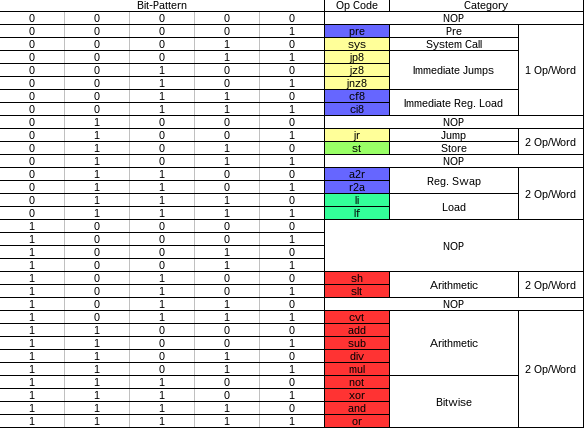
\includegraphics[width=\linewidth]{TACKY_encoding.png}
  \caption{TACKY Encoding}
  \Description{The encoding used in this project}
\end{figure}

TACKY will also be able to process both integer and floating point 16-bit instructions. To allow for int and float differentiation, our registers are tagged: 0 for integer and 1 for floating point. This means that each register is actually 17 bits. Because our VLIW is only 16 bits, we can only interpret 8-bit constants. To work up to 16 bits, we have an instruction called “pre” that is used to load the first half of a 16-bit constant in. This value is then prepended to the immediates of other instructions that take 8 bits.

To process our instructions, we implemented a five-stage pipeline. The stages are as follows: Instruction Fetch, Register Read, ALU/MEM, ALU 2, Register Writeback. In between each stage, we have registers which take the outputs of one stage and temporarily stores it for the next stage. These stages respect the principle of "owner computes"; how registers are written to are controlled by only one stage; other stages which need to change the value of a register not controlled by it set flags to indicate to the owning stage that the value needs to change. 

\subsection{Stage 0: Instruction Fetch}
In our Instruction Fetch stage, an instruction is fetched from memory and neccesary stalls are detected and initiated if needed. The instruction is determined by a PC register, which get its next value from either an incrementer or a value given to it by the write back stage (mentioned further below), which it selects based on both a jump flag and if the processor is stalling for a dependency. This value is used to access the instruction memory, obtaining the next instruction that is written to a buffer for the next stage. This stage also utilizes logic attached to the registers of subsequent stages and the newly decoded instruction to decide the number of NOPs to push through to the next stage in order to resolve issues of dependencies and flow control. These are detailed more in the "Dependencies and Jump Handling" section.

\subsection{Stage 1: Register Read}
In our Register Read stage, we check the instructions being used in the operations we need to perform and fetch the values of the appropriate registers. In addition, we also perform the pre operation. The register values fetched are determined by the registers indicated in the instruction. The accumulator registers are always fetched, as this is a common occurence, but whether it is used is left to the subsequent stages. The pre instruction is completed in this stage, as the value to store is an immediate value which is available as soon as the instruction reaches this stage. This helps eliminate the pre register as a potential source of dependencies for instrucitons which use an immediate value. Immediate values are also formed in this stage and passed through subsequent stages as needed. The writeback stage is the only stage which direclty uses these values, but it is still passed to the stages between to keep the value and respective instruction in the same stage and avoid potential timing issues.  The instruction is passed on to the next stage, as well.

\subsection{Stage 2: ALU / Data Memory}
In our ALU/MEM stage, we have two ALUs. There are two goals for these ALUs: to perform arithmetic operations on the register values and to load from and store to memory. Each receive the instruction word, and the values of the registers it would be concerned about. If the instruction word had an immediate, it was fed to the first ALU and the second ALU does nothing. Most instructions will finish in this stage, with the exceptions of load float, load int, and floating-point divide. Load float and load int will read the 16-bit value from memory. Floating point divide will read from the reciprocal lookup table. All inputs to this stage are transferred to the next stage. An intermediate "out value" is also transferred to the next stage.

\subsection{Stage 3: ALU2}
In our ALU 2 stage, we finish up the operations that we didn’t finish in the previous stage. Again, there are two ALUs, and we receive the same things as input as the first stage of ALUs. In addition, we receive the intermediate value. This intermediate value is going to be the output for most instructions. For load float, we prepend a 1 to the value we read to signify that it is a float. For load int, we prepend a 0 instead. For floating point divide, we multiply the value from the lookup table by the accumulator. Again, we pass the instruction word, the register values, and the alu generated values to the next stage.

\subsection{Stage 1: Write Back}
In our Writeback stage, the results from the previous stages are collected and selectively stored based on the current instruction. These values include ALU results, data memory results from li and lf instrucitons, and an immediate value determined in the Register Read stage. This stage also handles the logic for determining if a conditional jump is taken or not. Register stores are written directly to the register file, where as values to be written to pc are stored in a buffer register. A flag is set in the event of a jump to allow the Instruction Fetch stage to determine whether the pc register needs to be incremented or set to the value this stage wrote to the buffer register. 

\subsection{Dependencies and Jump Handling}
Because our processor is pipelined, the effects of a previous instruction may not have taken effect when we begin processing the next one. For example, if two sequential instructions both read and modify the same register, the second instruction would read the old register value before the first instruction would update it. To solve this issue, we need to stall stages of our pipeline.

To check whether we need to stall, we first look at the instruction we are about to process, and we determine which registers are being read for this type of instruction. The registers and accumulators that the fetched instruction reads from are compared to the registers and accumulators that are written to in the following three stages. This is achieved using special decoder modules that look at the instruction and output the register numbers that are being read/written or don't care values if not applicable. If a common register is being read from and written to across stages, it is considererd a dependency. Four case statements in the Instruction Fetch stage check for any matches between registers written to in the other stages and the register being read from in the Instruction Fetch stage. Once matches are found, their stage locations are compared. Stages that are farther away from the Register Writeback stage require more NOPs to be padded. Therefore, the number of NOPs to pad is the number related to whichever dependency is farthest from the Writeback Register. This remains true for instances in which multiple dependencies happen across stages. To stall, we output nops for the next X clock cycles and freeze the pc. X is dependent on which stage we caught the dependency. 3 for Reg Read stage, 2 for ALU/MEM stage, and 1 for Writeback stage. If multiple dependencies occur across stages, the largest number of NOPs is used. Because we freeze the pc for this time, we will execute the correct instruction after getting through the nops. In addition to register dependencies, we also stall if we detect a jump instruction. For jumps, we stall until the instruction gets to the Writeback stage, so that if we need to jump, it will modify the pc. 

\subsection{Halting}
To handle the sys halting properly, we detected the instruction at the Instruction fetch stage. After this, NOPs were pushed into the pipeline following the sys instruction to avoid subsequent instructions from executing, while allowing ones still in the pipeline to complete. Once sys reaches the Write Back stage, the halt flag on the proccessor is set, which causes the clk signal to stop. 

%How to include a picture in this format
%\begin{figure}[h]
% \centering
%  \includegraphics[width=\linewidth]{}
%  \caption{}
%  \Description{}
%\end{figure}

\section{Testing}
Our test cases are included in a separate file called "testcases.txt". Test cases were written to cover as many memory, jump, and integer arithmetic instructions as possible. Operations involving floating point were left out, since we are not responsible for making sure that the floating point modules operate correctly. The instructions not tested outside of floating point is jr, li, and st.  The is set up to first test immediate register loads and jumps, followed by every other instruction fitting the criteria mentioned earlier. This is done by having sys operations after conditional jumps. These conditional jumps are used to test registers which hold the results of some operation, if the jump is taking, the sys opertion is skipped, else the sys operation is run and causes the processor to halt.  

\section{Issues}
During testing, our processor could properly read and parse instructions until we reached a jump instruction followed by a sys instruction. We supplied the first stage with a jump flag and the pc to jump to, but because it was followed by a sys, our processor parsed the sys instead of jumping. This was likely due to the fact that the actual padding of NOPs was performed at the Register Read stage instead of at the Instruction fetch stage, which caused the next instruction to be visible to the components which decided halting. As a result, testing for whether the sys operation had instructions executing after it became difficult, but from what we've seen this appears to not be the case. Other instructions appear to operate normally.  

\end{document}
